\begin{figure}[H]
    \centering
    \begin{tabular}{|p{\textwidth/4} p{\textwidth/12} p{\textwidth/16} p{\textwidth/2}|}
        \hline
        \textbf{Name} & \textbf{Typ} & \multicolumn{2}{l|}{\textbf{Abgedeckte Anforderungen}} \\\hline
        Startbildschirm & Dialog & FA60 & Hauptmenü [Ansicht]\\\hline
        Hilfe & Dialog & FA65 & Hilfe [Ansicht]\\
        & & QA18 & Benutzerfreundlichkeit\\\hline
        Hotkey-Liste & Dialog & FA65 & Hilfe [Ansicht]\\
        & & FA68 & Hotkeys\\\hline
        Team ändern & Popup & FA63 & Team-Konfiguration importieren [Ansicht]\\
        & & FA15 & Teams\\
        & & FA54 & Quidditchtem-Konfiguration\\
        & & FA61 & Spiel beitreten [Ansicht]\\\hline
        Beenden & Popup & & \\\hline
        Spielstart fehlgeschlagen & Popup & QA16 & Zuverlässigkeit\\\hline
        Verlassen & Popup & &\\\hline
        Spielsuche & Dialog & FA61 & Spiel beitreten [Ansicht]\\
        & & FA55 & Netzwerkschnittstelle\\\hline
        Spielende & Dialog & FA62 & Spiel Ende [Ansicht]\\
        & & FA49 & Spielende\\\hline
        Beobachten & Dialog & FA66 & Beobachter [Ansicht]\\\hline
        Verbindungsabbruch & Dialog & QA16 & Zuverlässigkeit\\
        & & QA17 & Robustheit\\\hline
        Pause & Dialog & FA69 & Pausieren\\\hline
    \end{tabular}
\end{figure}
\begin{figure}[H]
    \centering
    \begin{tabular}{|p{\textwidth/4} p{\textwidth/12} p{\textwidth/16} p{\textwidth/2}|}
        \hline
        Spiel & Dialog & FA64 & Spiel[Ansicht]\\
        & & FA1 & Spielfeld\\
        & & FA2 & Mittelkreis\\
        & & FA3 & Mittelzelle\\
        & & FA4 & Hüterzone\\
        & & FA5 & Zelle\\
        & & FA6 & Torring\\
        & & FA8 & Punkte erzielen\\
        & & FA10 & Ball\\
        & & FA11 & Quaffel [Ball]\\
        & & FA12 & Klatscher [Ball]\\
        & & FA13 & Goldener Schnatz [Ball]\\
        & & FA14 & Besen\\
        & & FA16 & Spielfiguren\\
        & & FA17 & Jäger\\
        & & FA18 & Treiber\\
        & & FA19 & Hüter\\
        & & FA20 & Sucher\\
        & & FA31 & Fans\\
        & & FA32 & Elfen [Fantyp]\\
        & & FA33 & Kobolde [Fantyp]\\
        & & FA34 & Trolle [Fantyp]\\
        & & FA35 & Niffler [Fantyp]\\
        & & FA36 & Schiedsrichter\\
        & & FA44 & Runde\\
        & & FA46 & Spielerphase\\\hline
    \end{tabular}
\end{figure}

\subsubsection{Startbildschirm}
\begin{figure}[H]
	\centering
	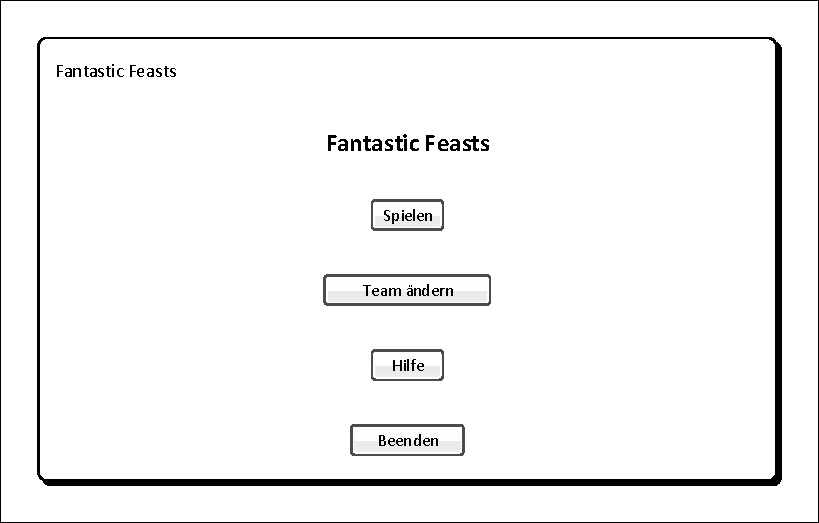
\includegraphics[scale=0.8]{images/Startbildschirm.pdf}
\end{figure}

Dieser Dialog erscheint nach Start der Anwendung. Der "Spielen"-Button öffnet den Spielsuche-Dialog. Der "Team ändern"-Button öffnet das 'Team ändern'-Popup. Der "Hilfe"-Button öffnet den Hilfe-Dialog. Der "Beenden"-Button öffnet ein Bestätigungs-Popup und beendet bei positiver Antwort die Anwendung.

\subsubsection{Spielsuche}
\begin{figure}[H]
	\centering
	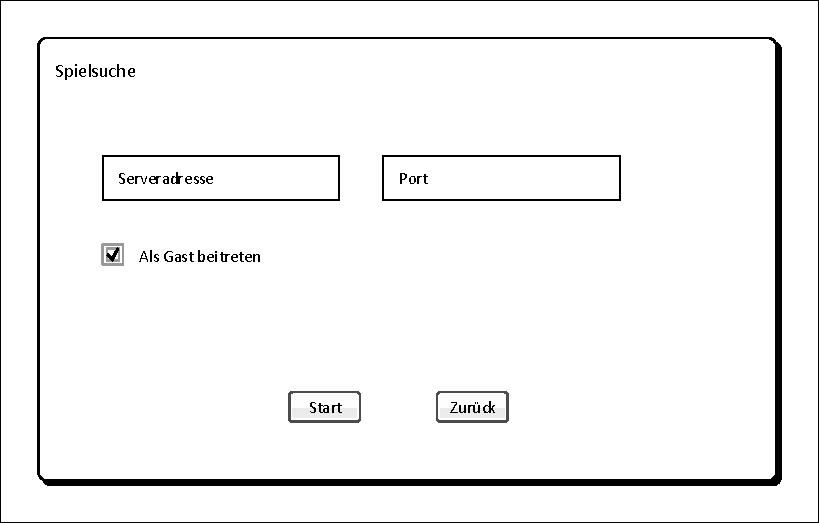
\includegraphics[scale=0.8]{images/Spielsuche.pdf}
\end{figure}

Der Benutzer gibt zuerst die Adresse und den Port des Spielservers und, mit dem er sich verbinden möchte. Wenn er die Partie beobachten will, hakt er "Als Gast beitreten" ab. Drückt er anschließend auf den "Start"-Button, versucht sich der Client mit dem angegebene Server zu verbinden. Mit dem "Zurück"-Button kann man zurück auf den Startbildschirm gelangen.
	
\subsubsection{Hilfe}
\begin{figure}[H]
	\centering
	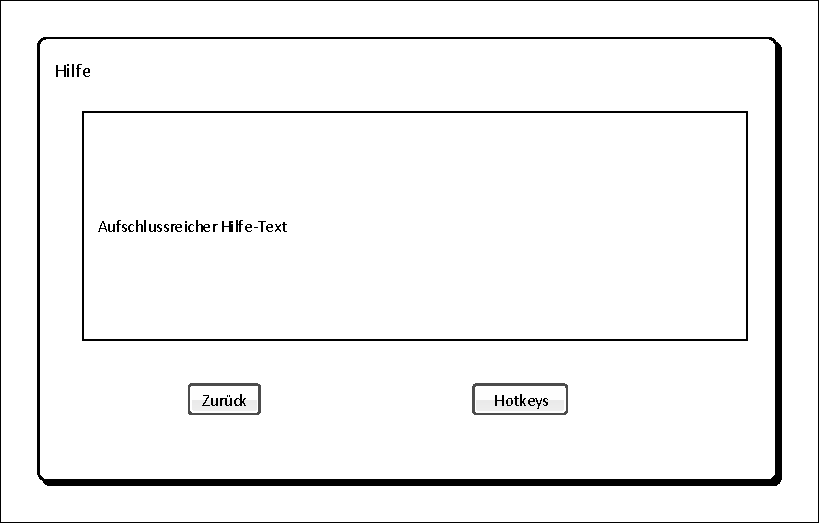
\includegraphics[scale=0.8]{images/Hilfe.pdf}
\end{figure}

In einem großen Textfeld, gegebenenfalls mit Scrollbar, wird ein Hilfetext angezeigt. Der "Zurück"-Button öffnet den Startbildschirm, der "Hotkey"-Button den Hotkey-Dialog.

\subsubsection{Hotkeys}
\begin{figure}[H]
	\centering
	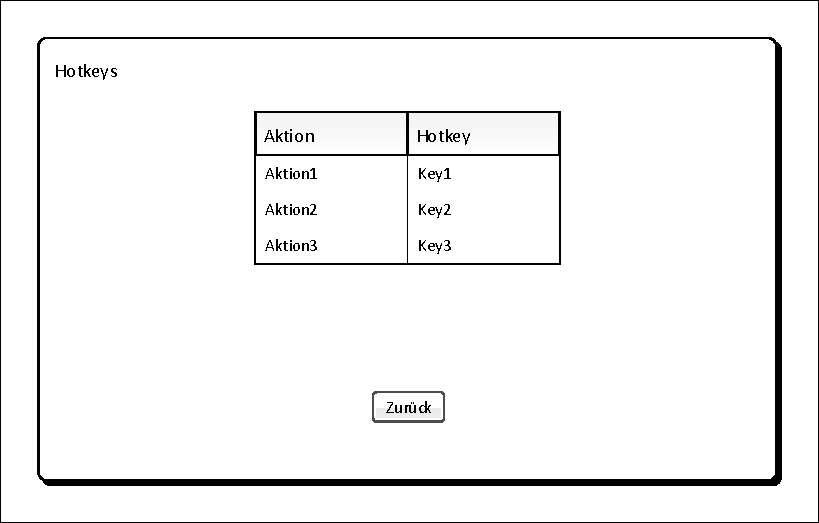
\includegraphics[scale=0.8]{images/Hotkeys.pdf}
\end{figure}

Hier werden alle verfügbaren Hotkeys in Tabellenform aufgelistet. Der "Zurück"-Button öffnet den Hilfe-Dialog.

\subsubsection{Team ändern}
\begin{figure}[H]
	\centering
	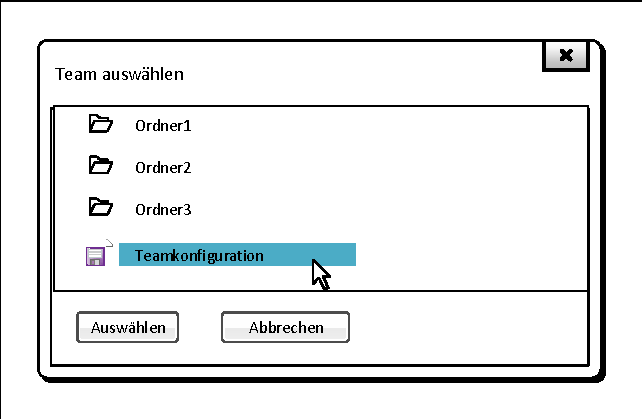
\includegraphics[scale=0.8]{images/Teamauswahl_Popup.pdf}
\end{figure}

In diesem Popup kann der Benutzer durch sein Dateisystem navigieren und eine JSON-Datei auswählen. Hat er eine gültige Datei ausgewählt und betätigt den "Auswählen"-Button, wird das Popup geschlossen und die Team-Konfiguration, mit der er ins Spiel kommt, ist die, die er ausgewählt hat. Der "Abbrechen"-Button schließt das Popup und es werden keine Änderungen vorgenommen.

\subsubsection{Bestätigungsaufforderung}
\begin{figure}[H]
	\centering
	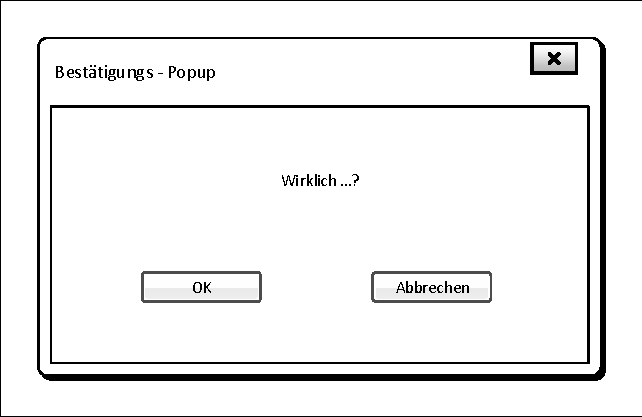
\includegraphics[scale=0.8]{images/OK_Popup.pdf}
\end{figure}

Dieser Aufbau wird für die Popups "Beenden" und "Verlassen" verwendet. Der "Abbrechen"-Button schließt das Popup und der Benutzer gelangt zurück in den Dialog, in dem er vor Öffnen des Popups war. Der "OK"-Button führt dazu, dass eine Aktion ausgeführt wird.

\subsubsection{Fehler}
\begin{figure}[H]
	\centering
	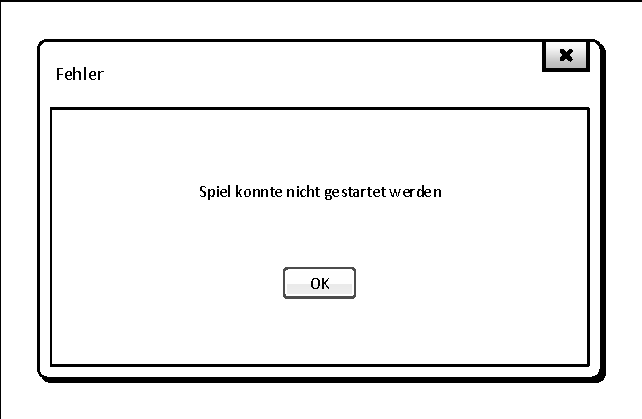
\includegraphics[scale=0.8]{images/Fehler_Popup.pdf}
\end{figure}

Dieser Aufbau wird für das Popup "Spielstart fehlgeschlagen" verwendet. Der angezeigt Text richtet sich nach dem aufgetretenen Fehler. Der "OK"-Button schließt das Popup.

\subsubsection{Pause}
\begin{figure}[H]
	\centering
	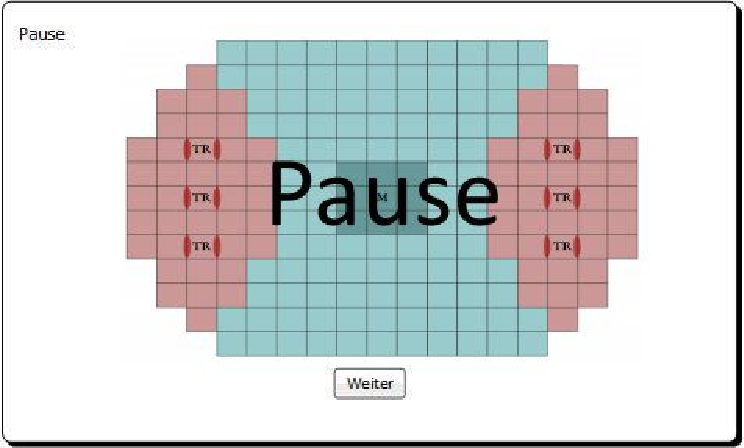
\includegraphics[scale=0.8]{images/Pause.pdf}
\end{figure}

Wird angezeigt, wenn das Spiel von einem Spieler pausiert wird. Der "Weiter"-Button setzt die Partie fort und kann nicht von einem Gast betätigt werden.

\subsubsection{Verbindungsabbruch}
\begin{figure}[H]
	\centering
	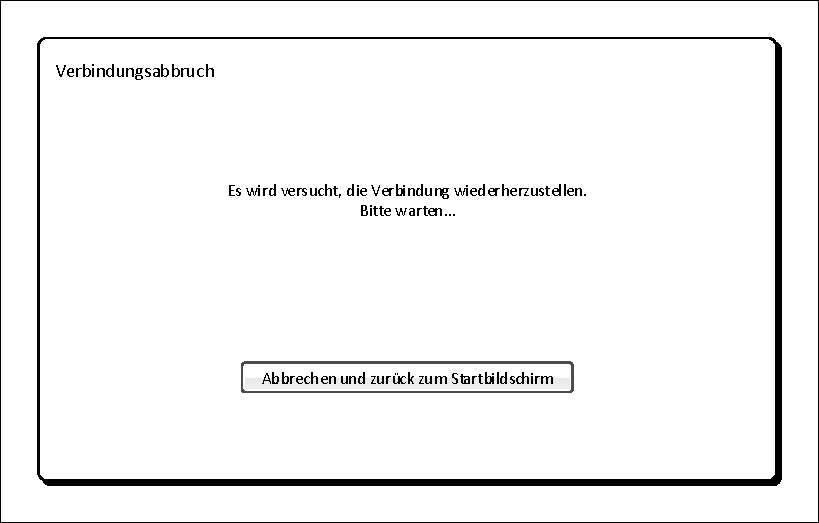
\includegraphics[scale=0.8]{images/Verbindungsabbruch.pdf}
\end{figure}

Im Falle eines Verbindungsabbruchs zwischen Client und Server wird dieser Dialog angezeigt. Wird die Verbindung wiederhergestellt, gelangt der Benutzer automatisch wieder zurück in den vorherigen Dialog. Alternativ kann er durch betätigen des Buttons zum Startbildschirm gelangen. Ist er ein Spieler, kann er die Partie nicht weiterführen und sein Gegner gewinnt nach Ablauf einer Zeitdauer die Partie.

\subsubsection{Spielende}
\begin{figure}[H]
	\centering
	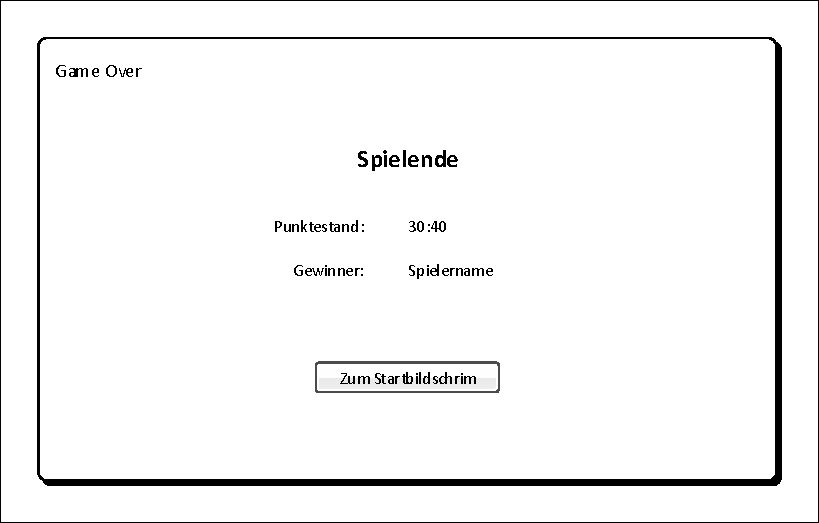
\includegraphics[scale=0.8]{images/Spielende.pdf}
\end{figure}

Bei Spielende wird dieser Dialog geöffnet. Hier werden der Punktestand bei Spielende und der Name des Gewinners angezeigt. Der Button öffnet den Startbildschirm-Dialog